\section{Theoretische Grundlagen}
\label{sec:grundlagen}
%zugrundeliegende Theorien und Modelle
% Definitionen
% Stand der Technik, Normen und Standards, Wirtschaftliche Aspekte
% persönliche Positionierung

\subsection{Definition und Gliederung zu Verdickungsmitteln}

In der Farben- und Putzindustrie werden Verdickungsmittel als rheologische Additive bezeichnet. Sie erhöhen die Viskosität von Flüssigkeiten und ändern somit ihre rheologischen Eigenschaften, welche die Auftragungs-, Fließ- und Verlaufseigenschaften von Farben und Putzen bestimmen. Verdickungsmittel kommen jedoch auch in der Lebensmittelchemie oder Pharmazie zum Einsatz. Je nach dem welche Anforderungen an das Verdickermittel gestellt werden, unterscheiden sich diese in ihrer Zusammensetzung (siehe Abb. \ref{fig:verdicker_einteilung}). \cite{Brock.2009}

\begin{figure}[h!]
	\centering
	\begin{forest}
		forked edges,
		for tree={draw,align=center,edge={-latex}}
		[Verdickungsmittel, for children={fit=band}
			[Anorganisch]
			[Organisch, for children={fit=band}
				[Niedermolekular]
				[Synthetisch]
				[Natürlich, for children={fit=band}
					[Natürlich (abgewandelt)]
					]	
			]	
		]
	\end{forest}	
	\caption{Einteilung von Verdickungsmitteln nach Zusammensetzung \cite{Brock.2009}}
	\label{fig:verdicker_einteilung}
\end{figure}
\FloatBarrier

Je nach Verdickungsmittel können verschiedene Effekte wie Gelbildung, Solvatation, Ausbildung von Netzstrukturen, Coulomb-Kräfte, Quellung und Wasserstoff- Brückenbindungen, sowie deren gegenseitige Einflussnahme die Erhöhung der Zähflüssigkeit bewirken. \cite{Brock.2009} \\
Betrachtet man speziell die sogenannten assoziativen Verdickungsmittel lassen sich diese den Gruppen der abgewandelten, natürlichen Verdicker und den synthetischen Verdickern zuordnen.  Sie spezifizieren sich gegenüber anderen Verdickertypen darin, dass sie neben hydrophilen Gruppen auch hydrophobe End- und Seitengruppen enthalten, welche dem Verdickungsmittel einen Tensidcharakter verleihen. Deshalb bestehen assoziative Verdicker unteranderem aus hydrophob modifizierten Polymerstrukturen (siehe Abb. \ref{fig:assoziativ_einteilung}).

\begin{figure}[h!]
	\centering
	\begin{forest}
		forked edges,
		for tree={draw,align=center,edge={-latex}}
		[Assoziativverdicker
		[hydrophob \\ modifizierte \\ Polyacrylate]
		[hydrophob \\ modifizierte \\ Celluloseether]
		[hydrophob \\ modifizierte \\ Polyether]
		[hydrophob \\ modifizierte \\ Polyacrylamide]
		[assoziative \\ Polyurethan-Verdicker]
		]
	\end{forest}	
	\caption{Einteilung von Assoziativ-Verdickern nach chemischer Struktur \cite{Brock.2009}}
	\label{fig:assoziativ_einteilung}
\end{figure}
\FloatBarrier
Diese strukturelle Eigenschaft der Assoziativ-Verdicker macht die Bildung von Micellen möglich und es treten neben der Quellung in der Wasserphase sogenannte "`Micellbrücken"' zwischen Latex-Teilchen der Bindemitteldisperion auf, welche eine zusätzlich Viskositätserhöhung bewirken. \cite{Brock.2009} \\
In Abbildung \ref{fig:struktur_puverdicker} ist eine schematische Struktur eines solchen assoziativen Polyurethan-Verdickers aufgeführt. Diese beispielhafte Struktur zeigt hydrophile, höher molekulare Polyethersegmente, welche über Urethan-Gruppen verbunden sind und durch hydrophobe Molekülgruppen verknüpft werden. \cite{Brock.2009}

\begin{figure}[h!]
	\centering
	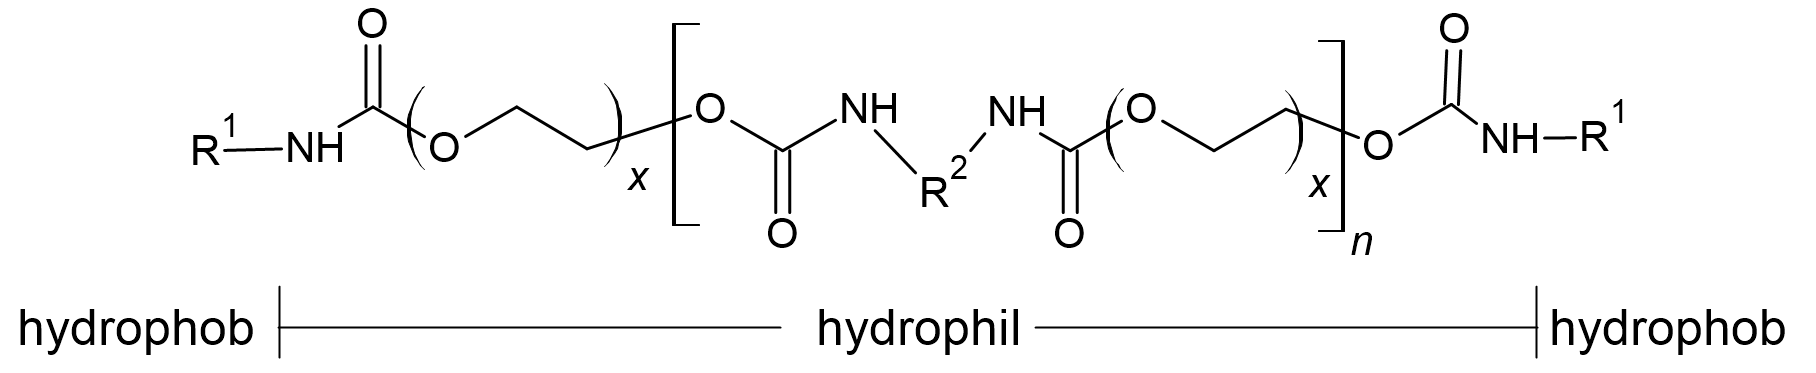
\includegraphics[width=0.75\textwidth]{img/verdicker_struktur}
	\caption{schematische Struktur eines assoziativen Polyurethan-Verdickers, \linebreak erstellt nach \cite{Brock.2009}}
	\label{fig:struktur_puverdicker}
\end{figure}
\FloatBarrier

Durch diesen Mix der hydrophoben und hydrophilen Strukturen wird der Tensidcharakter des Verdickungsmittels bestimmt und es ergeben sich Netzstrukturen mit assoziierten "`Micellbrücken"', wie in Abbildung \ref{fig: verdicker_anwendung} dargestellt. Zusätzlich ist zu erkennen, dass auch Wechselwirkungen mit bereits vorhandenen Tensidmolekülen in der Dispersion auftreten können und die Struktur somit weiter stabilisieren. \cite{Mezger.2016}

\begin{figure}[h!]
	\centering
	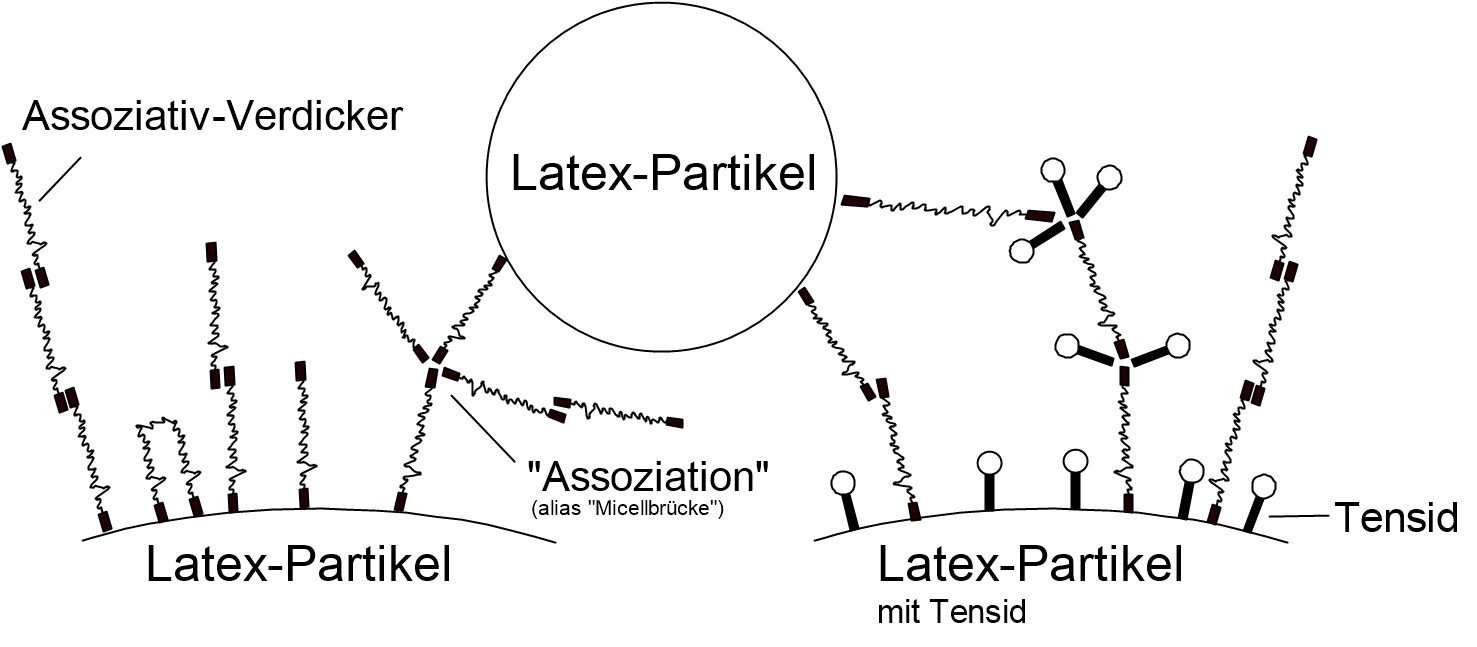
\includegraphics[width=0.75\textwidth]{img/verdicker_anwendung}
	\caption{Netzstruktur durch Verdickermittel in Latex-Dispersion (mit und ohne Tensid), \linebreak erstellt nach \cite{Mezger.2016}}
	\label{fig: verdicker_anwendung}
\end{figure}
\FloatBarrier

Aufgrund dieser ausgeprägten Netzstrukturen innerhalb des Verdickungsmittels ist es jedoch auch möglich, dass das Verdickungsmittel selbst eine hohe Viskosität aufweist. Dieser Punkt kann erheblichen Einfluss auf die großtechnische Verarbeitbarkeit des Additives haben und wird im weiteren Verlauf dieser Arbeit näher betrachtet. 

\subsection{Dosierung von Flüssigkeiten}

\subsubsection{Charakterisierung des Dosierstroms}
%\paragraph*{Rheologie von Fluiden}\\
Um den Dosierstrom einer Flüssigkeit charakterisieren,  ist es zunächst nötigt die Fließeigenschaften beschreiben zu können. Die Wissenschaft der Rheologie beschäftigt sich unter anderem mit dem Fließ- und Deformationsverhalten von Flüssigkeiten und teilt diese zunächst in \textsc{Newtonsche} und \textsc{Nichtnewtonsche} Fluide ein. Grundlage dieser Einteilung sind Untersuchungen von \textsc{Isaac Newton}, welcher sich bei konstanter Temperatur mit der Schergeschwindigkeit $D$ in Abhängigkeit von der Schubspannung $\tau$ beschäftigte. 
Das Ergebnis dieser Arbeit ist das \textsc{Newtonsche Fließgesetz} unter Gleichung \eqref{eq: newton}, welche den Fließwiderstand $\eta$ einer Flüssigkeit bei gegebener Temperatur als Stoffkonstante benennt. Dieser Fließwiderstand $\eta$ ist heute unter der Bezeichnung der dynamischen Viskosität bekannt.

\begin{equation}
	\label{eq: newton}
	\tau = \eta * D
\end{equation}
\begin{parameter}
	D 			& Schergeschwindigkeit\\
	\tau 		& Schubspannung\\
	\eta 		& Dynamische Viskosität\\
\end{parameter}

Es sei erwähnt, dass neben der dynamischen Viskosität auch eine kinematische Viskosität $\nu$ existiert. Diese beschreibt in Gleichung \eqref{eq:kivisko} jedoch lediglich das Verhältnis zwischen der dynamischen Viskosität und der Dichte eines Fluides.

\begin{equation}
	\label{eq:kivisko}
	\nu = \frac{\eta}{\rho}
\end{equation}
\begin{parameter}
	\nu 		& kinematische Viskosität\\
	\rho 		& Dichte\\
	\eta 		& Dynamische Viskosität\\
\end{parameter}

Schlussendlich gilt für die Einteilung der Fluide nach Gleichung \eqref{eq: newton}, dass alle Fluide, welche eine Linearität zwischen Schergeschwindigkeit und Schubspannung ohne Fließgrenze aufweisen als \textsc{Newtonsche} Fluide und diejenigen, die ein nicht-lineares Verhalten und/oder ein Verhalten mit Fließgrenze aufweisen als \textsc{Nichtnewtonsche} Fluide eingeordnet werden. Veranschaulicht wird dies in Abbildung\,\ref{fig: arten_fluide} mit einer Auswahl an verschiedenen Rheologieprofilen.

\begin{figure}[h!]
	\begin{minipage}[b]{0.475\textwidth}
		\includegraphics[width=\textwidth]{img/fluidarten}
		\caption{Fließkurven für verschiedene \linebreak Fluide, erstellt nach \cite{Holze.2010}}
		\label{fig: arten_fluide}
	\end{minipage}
	\hspace*{0.05\textwidth}
	\begin{minipage}[b]{0.475\textwidth}
		\includegraphics[width=\textwidth]{img/fluidarten2}
		\caption{Viskositätskurven für verschiedene Fluide, erstellt nach \cite{MunzingChemieGmbH.2018}}
		\label{fig: arten_fluide2}
	\end{minipage}
\end{figure}
\FloatBarrier

%\paragraph*{Messmethoden zur Viskositätsbestimmung}
Zur Bestimmung der Viskosität müssen für ein \textsc{Newtonsches} Fluid laut Gleichung\,\eqref{eq: newton} die Schergeschwindigkeit $D$ und die Schubspannung $\tau$ bestimmt werden. Eine Möglichkeit hierfür ist die Nutzung eines sogenannten Rotationsviskosimeters. Allgemein beschreiben Rotationsviskosimeter einen Viskosimetertypen, bei dem die zu messende Flüssigkeit zwischen spezifisch geformten Körpern gebracht wird, von denen einer rotiert. Dabei tritt eine Scherung der Flüssigkeit auf und das aufgewendete Drehmoment am Viskosimeter wird gemessen. Neben Rotationsviskosimetern sind auch weitere Viskosimetertypen wie Kappilarviskoskosimeter und Fallkörperviskosimeter bekannt. Diese unterscheiden sich neben dem Aufbau gegenüber dem Rotationsviskosimeter beispielsweise auch darin, dass sie im Regelfall die Viskosität von \textsc{Nichtnewtonschen} Fluiden nicht ausreichend untersucht werden kann. \cite{ROMPPRedaktion.2008}

%\paragraph*{Bestimmung der Strömungsform}
Nachdem die Viskosität bestimmt ist, lässt sich nun der Dosierstrom des Verdickermittels entsprechend seiner Strömungseigenschaften beschreiben. Hier für wird die sogenannte \textsc{Reynoldszahl} bestimmt. Sie ist eine dimensionslose Kennzahl und beschreibt das Verhältnis zwischen Trägheitskräften zu Reibungskräften in strömenden Flüssigkeiten und ist für durchströmte Rohrleitungen unter Gleichung\,\eqref{eq: reynolds} definiert. \cite{Foth.2014}

\begin{equation}
	\label{eq: reynolds}
	Re = \frac{d_H*\rho*\overline{u}}{\eta}
\end{equation}
\begin{parameter}
	Re 			& 	\textsc{Reynoldszahl} \\
	\eta 		& dynamische Viskosität des Fluids\\
	\rho 		& Dichte des Fluids\\
	d_H			&	hydraulischer Rohrdurchmesser\\
	\overline{u} & mittlere Strömungsgeschwindigkeit\\
\end{parameter}

Anhand der \textsc{Reynoldszahl} lässt sich nun mithilfe der Tabelle \ref{tab:stromung_reynolds}, die jeweilige Strömungsform zuordnen. Diese Zuordnung ist wichtig, da sich je nach Strömungsform unterschiedliche Einflussgrößen auf den Druckverlust somit auf die Auslegung der Dosierung ergeben. Beispielsweise hat für eine laminare Strömung die Wandrauigkeit der Leitung keinen Einfluss mehr, wohin gegen sie in turbulenten Strömungen maßgebliche Druckverluste hervorrufen kann. In laminaren Strömungen überwiegt hierbei der glättende Einfluss der Viskosität gegenüber den Rohrunebenheiten, während in turbulenten Strömungen weitere Wirbel erzeugt werden. \cite{Bschorer.2018}

% Table generated by Excel2LaTeX from sheet 'Daten'
\begin{table}[h!]
	\renewcommand*{\arraystretch}{1.2}
	\centering
	\caption{Strömungsformen und ihre Reynoldszahlen \cite{Foth.2014}}
	\label{tab:stromung_reynolds}
	%\resizebox{10.5cm}{!}{
		\begin{tabulary}{1.0\textwidth}{C|CCC}
			\hline
			\textbf{Strömungsform} & \textbf{Laminar} & \textbf{instabiler Bereich} & \textbf{Turbulent}\\
			\hline
			\textbf{Reynoldszahl} &	$< 2300$ & $2300$ bis $4000$& $>4000$\\
			\hline			
		\end{tabulary}
		%}
\end{table}%
\FloatBarrier

Nach der Bestimmung der Reynoldszahl lässt sich nun mit Hilfe des \linebreak \textsc{Nikuradse-Colebrook-Moody}-Diagramms, nachfolgend \textsc{Moody}-Diagramm genannt, die Rohrreibungszahl $\lambda$ bestimmen (siehe Abb. \ref{fig:moody}). Diese Rohrreibungszahl ist eine dimensionslose Kennzahl und kann zweckmäßig in Gleichung \eqref{eq:druckverlustbeiwert} eingesetzt werden. Somit ist es möglich den dimensionslosen Druckverlustbeiwert $\zeta_R$ für gerade Rohrleitungen zu bestimmen und ermöglicht daraufhin die Berechnung des durch Reibung verursachten Druckverlustes $\Delta p$ auf Basis der erweiterten \textsc{Bernoulli}-Gleichung \eqref{eq:druckverlust_zeta}. \cite{Bschorer.2018}

\begin{equation}
	\label{eq:druckverlustbeiwert}
	\zeta_R = \lambda * \frac{L}{d}
\end{equation}
\begin{equation}
	\label{eq:druckverlust_zeta}
	\Delta p = \frac{1}{2}*\zeta_R*\rho*\overline{u}^2
\end{equation}
\begin{parameter}
	\zeta_R		& Druckverlustbeiwert für gerade Rohrstrecken\\
	L 			& Rohrleitungslänge\\
	d			& Rohrdurchmesser\\
	\Delta p	& Druckverlust \\
	\rho 			& Dichte des Fluids\\
	\overline{u} 	& mittlere Strömungsgeschwindigkeit\\
\end{parameter}


\begin{figure}[h!]
	\centering
	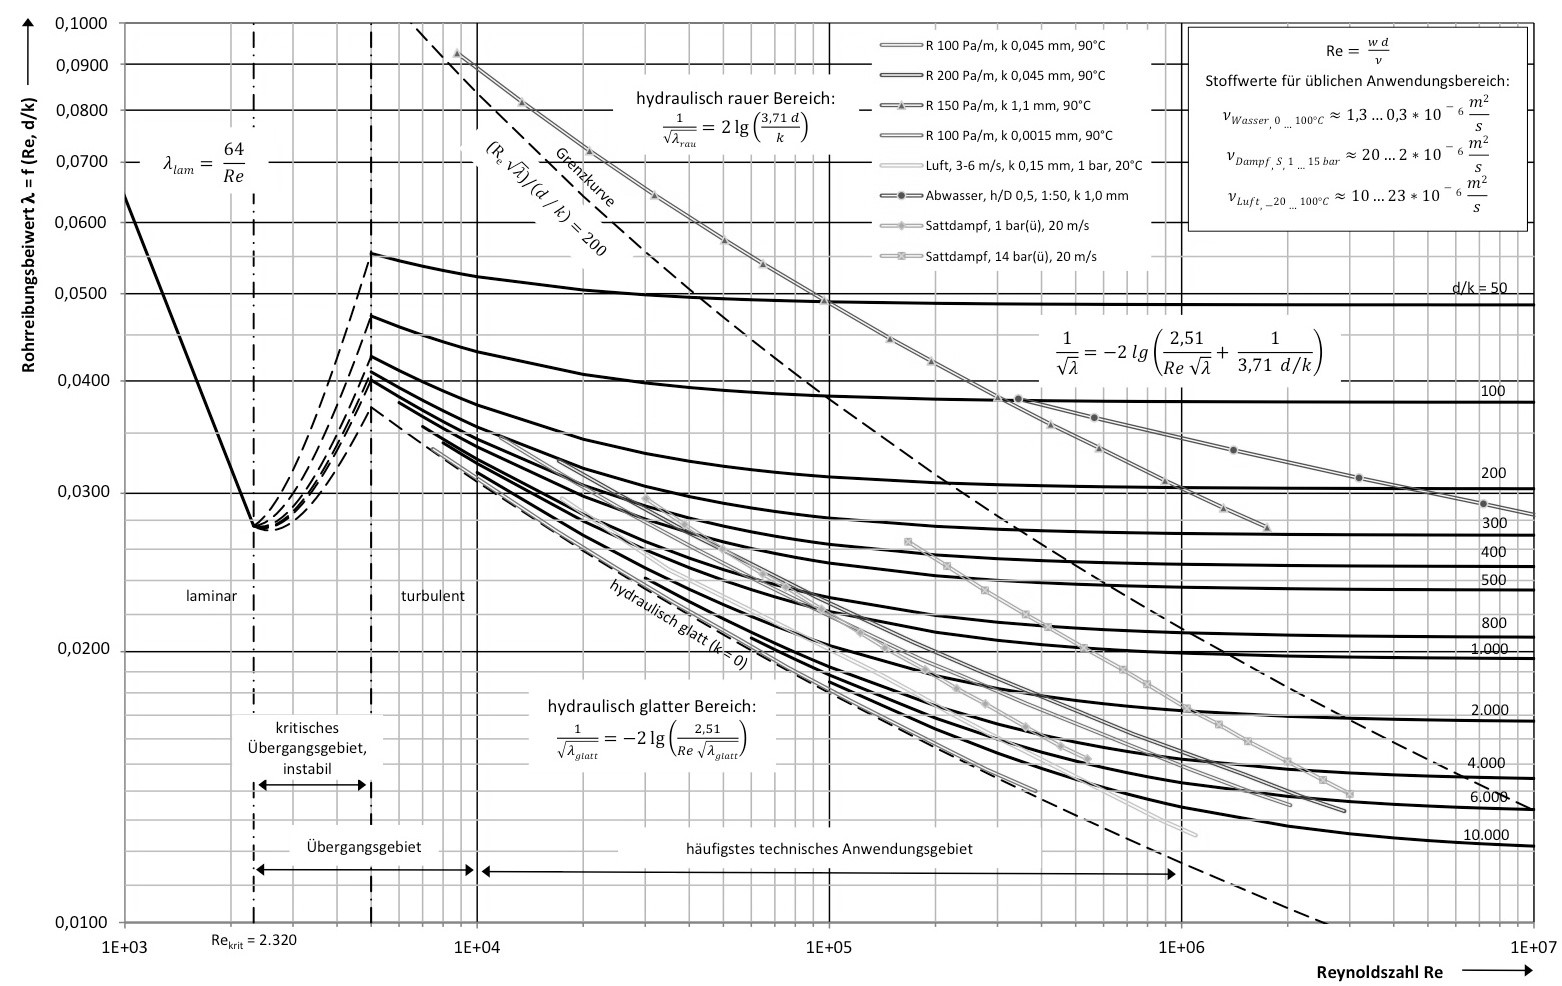
\includegraphics[width=1.0\textwidth]{img/R_Rohrreibungsbeiwert.jpg}
	\caption{\textsc{Nikuradse-Colebrook-Moody}-Diagramm \cite[\ccbysa]{Msimca.2017}}
	\label{fig:moody}
\end{figure}
\FloatBarrier
%Ende

%\paragraph*{Gesetz von  \textsc{Hagen}-\textsc{Poiseuille}}
Liegt für eine nicht-kompressible Flüssigkeit eine laminare Strömung vor, so ist es möglich die zuvor beschriebene Vorgehensweise zu vereinfachen und den auftretenden Druckverlust in einer geraden Rohrleitung direkt mit dem Gesetz von \textsc{Hagen}-\textsc{Poiseuille} zu bestimmen.  Der Druckverlust wird hierbei in Abhängigkeit vom Volumenstrom, der Rohrleitungslänge, des Rohrdurchmessers und der Viskosität berechnet. Die Definition des Gesetzes, aufgelöst nach dem Druckverlust, findet sich unter Gleichung \eqref{eq:hagen}. \cite{Foth.2005}

\begin{equation}
	\label{eq:hagen}
	\Delta p  = \frac{8*\eta*L*\dot{V}}{r^4*\pi}
\end{equation}
\begin{parameter}
	\Delta p	& Druckverlust \\
	\eta 		& dynamische Viskosität des Fluids\\
	\dot{V}		& Volumenstrom des Fluids\\
	r			& innerer Radius der Rohrleitung\\
	L 			& Rohrleitungslänge\\
\end{parameter}

Da das Gesetz von \textsc{Hagen}-\textsc{Poiseuille} bereits im \textsc{Moody}-Diagramm enthalten ist, können beide Vorgehensweisen genutzt werden um die jeweils andere Rechnung zu überprüfen. Sollen Rohrleitungseinbauten wie Armaturen, Ventile oder Bogenstücke einberechnet werden, vereinfacht jedoch aufgrund von tabellierten Druckverlustbeiwerten möglicher Einbauten die erweiterte \textsc{Bernoulli}-Gleichung die Berechnung des gesamten reibungsbedingten Druckverlustes.

\subsubsection{Dosierpumpen}
Da Flüssigkeiten keine hohen Abweichungen der Dichte in Abhängigkeit von geringen Druck- und Temperaturschwankungen aufzeigen, kann selbst eine volumenbegrenzte Dosierung sehr genau sein. Durch die fest definierten Abgrenzungsräume ("`Kammern"') wird eine solche volumenbegrenzte Flüssigkeitsdosierung in aller Regel mit rotierenden oder oszillierenden Verdränger-Dosierpumpen umgesetzt. Sie zeichnen sich im Vergleich zu Kreiselpumpen dadurch aus, dass die Förderhöhe weitestgehend unabhängig vom Förderstrom ist.  Da je nach Dreh- oder Hubzahl ein festes Volumen gefördert wird, eignen sie sich gut, wenn ein Dosierverfahren ohne weitere Messeinrichtung vorausgesetzt wird. Dennoch lassen SIe sich auch mit verschiedenen Messverfahren kombinieren, um so die Dosierung so genau wie möglich zu gestalten. Eine genaue Definition für den realen Förderstrom von Verdrängerpumpen findet sich unter Gleichung \ref{eq:pump_masse}. \cite{Ignatowitz.2015,Vetter.2002}

\begin{equation}
	\label{eq:pump_masse}
	\dot{m} = i*V_K*n*\rho*\eta_V
\end{equation}
\begin{parameter}
	\dot{m}		& Fördermassenstrom \\
	i 			& Anzahl der verdrängbaren "`Kammern"'\\
	V_K			& Kammervolumen\\
	n			& Drehzahl bzw. Hubfrequenz\\
	\rho		& Dichte der Flüssigkeit\\
	\eta_V 		& volumetrischer Wirkungsgrad\\
\end{parameter}

Da in der Realität die rein geometrische Volumenabgrenzung durch die "`Kammern"' der Pumpe vom messbaren Förderstrom abweicht wird in Gleichung\,\eqref{eq:pump_masse} der volumetrische Wirkungsgrad $\eta_V$ als Korrekturfaktor genutzt. Dieser unter Gleichung\,\eqref{eq:vol_wirkungsgrad} definierte Wirkungsgrad wird von den Eigenschaften des Fluids, sowie von den Betriebsbedingungen und beschreibt dabei das Verhältnis zwischen dem realen Förderstrom $\dot{V}$ und dem theoretisch, geometrischen Förderstrom $\dot{V}_{\text{theo}}$. \cite{Vetter.2002}

\begin{equation}
	\label{eq:vol_wirkungsgrad}
	\eta_V = f(\Delta p, \rho, \nu, E_{\text{geo}}) = \frac{\dot{V}}{\dot{V}_{\text{theo}}}
\end{equation}
\begin{parameter}
	\dot{V}	& realer Volumenstrom \\
	\dot{V}_{\text{theo}}	& theoretischer Volumenstrom \\
	\Delta p 			& Differenzdruck\\
	\nu			& kinematische Viskosität der Flüssigkeit\\
	\rho		& Dichte der Flüssigkeit\\
	E_{\text{geo}} 	& pumpenspezifische Geometrie\\
\end{parameter}

Verursacht werden diese Abweichungen vom theoretischen Förderstrom durch Leckage- und Elastizitätseinflüsse, welche hauptsächlich durch den von der Pumpe geforderten Differenzdruck entstehen. Der Arbeitsraum der Dosierpumpe ist daher so starr und dicht wie möglich auszuführen.
Da neben den Fluid- und den Betriebsbedingungen auch die Bauart bzw. die Pumpengeometrie Einfluss auf den volumetrischen Wirkungsgrad nimmt, ist es wichtig sich genauer mit den verschiedenen Arten der Verdrängungspumpen auseinanderzusetzen. Auch Einflüsse, die die Einbindung und Handhabung in der Produktion betreffen, können entscheidend für die Wahl des Pumpentyps sein.\\

Zum einen gibt es die Kategorie der oszillierenden Dosierpumpen. Diese Pumpen kennzeichnen sich dadurch, dass sie ein Fluid durch Hubbewegungen eines Verdängerkörpers fördern. Dieser verdrängende Körper kann bei einer klassischen Pumpe ein zylindrischer Kolben sein, jedoch sind heutzutage vorrangig Membranpumpen im Einsatz bei der das Fördermedium durch eine spezielle Membran getrennt ist (vgl. Abbildung \ref{fig:kolben_membran_pumpe}). 

\missingfigure{Kolben- und Membranpumpe}

Die im Betrieb nutzbaren Stellgrößen bei diesen Pumpen konzentrieren sich aufgrund ihrer Funktionsweise auf die Hublänge und die Hubfrequenz. Durch den geometrisch genau definierten Hubraum und weitestgehend Leckfreien Pumpenventilen und Kolbenabdichtungen, eigenen sich oszillierende Dosierpumpen am günstigsten für die Flüssigkeitsdosierung. Durch das Hubweise fördern der Flüssigkeit ergibt sich jedoch ein digitaler Charakter im Förderstrom. Somit eignen sich diese Pumpen lediglich für diskontinuierliche Dosierung mittels Hubzählung. Der Massenstrom der sich daraus für eine einzylindrige Kolbenpumpe ergibt, ist unter Gleichung \eqref{eq:oz_masse} zu finden. \cite{Vetter.2002}

\begin{equation}
	\label{eq:oz_masse}
	\dot{m} = h_K*A_K*n*\rho*\eta_V
\end{equation}
\begin{parameter}
	\dot{m}		& Fördermassenstrom \\
	h_K			& Hublänge\\
	h_K			& Kolbenquerschnitt\\
	n			& Hubfrequenz\\
	\rho		& Dichte der Flüssigkeit\\
	\eta_V 		& volumetrischer Wirkungsgrad\
\end{parameter}

%\paragraph*{rotierende Verdrängerpumpen}
Die Kategorie der rotierenden Dosierpumpen ist im Vergleich zu oszillierenden Dosierpumpen deutlich fassettenreicher. Das hierbei genutzte Verdrängervolumen basiert auf Maßtoleranzen, Spaltmaßen und Elastizitäten des Pumpraumes, welches durch Rotation der Verdrängersystems gefördert wird. Aufgrund dieser Toleranzen treten in rotierenden Verdrängerpumpen für niedrigviskose Flüssigkeiten merkliche, innere Leckagen auf und sind damit weniger genau als oszillierende Verdrängerpumpen. Sie eignen sich daher hauptsächlich für viskose Fluide. Eine Auswahl an typischen, rotierenden Dosierpumpen ist unter Abbildung \ref{fig:rotat_pumpe} dargestellt.

\missingfigure{Bilder Rotationspumpen ergänzen}

Hauptstellgröße dieser Pumpenart ist die Drehzahl. Ebenso wie die Hublänge/Hubfrequenz oszillierender Verdrängerpumpen besteht bei rotierenden Verdrängerpumpen eine direkte Proportionalität zwischen Drehzahl und Förderstrom. Eine einheitliche Charakteristik des Förderstroms lässt sich für diese Pumpen nicht definieren, da sich trotz Rotationsprinzip die Förderweisen stark unterscheiden. So weisen weißen beispielsweise Schlauchpumpen im Vergleich zu Zahnradpumpen eine viel deutlichere Pulsation des Förderstroms auf obwohl beide Pumpe den Rotationspumpen zugeordnet werden. Demnach lässt sich auch der Dosierstrom lediglich allgemein wie in Gleichung \eqref{eq:roations_strom} dargestellt beschreiben. Je nach Pumpentyp lässt dann sich die Ausführung der geometrischen Volumenabgrenzung detaillierter ausführen. \cite{Vetter.2002}

\todo[inline]{fehlender TVergleich zwischen verschiedenen Pumpentypen}

\missingfigure{Tabelle mit vergleich der Pumpen aus Gerhard Vetter}


\subsubsection{Ermittlung des Dosierstroms}
\paragraph*{Radarfüllstandsmessung}
\paragraph*{Coriolis-Massendurchflussmesser}
\paragraph*{Volumetrischer Verdränger}
\paragraph*{Waage mit Wägezellen}
\paragraph*{Durchflusskurve der Pumpe}

\subsection{Chemische Produktion und Prozesssicherheit}
\subsubsection{Produktionsweisen in der Chemie}
\subsubsection{Industrielle Gebinde für Flüssigkeiten}
Um ein Edukt neu in die Produktion einzubinden sind, nicht nur die chemisch-physikalischen Eigenschaften relevant. Auch der Aspekt der Gebindeform ist maßgeblich für die Einfügung des Eduktes in den Produktionsablauf. Für flüssige Edukte sind im Tagesgeschäft der \textsc{Alberdingk Boley Leuna GmbH} hauptsächlich Kunststoff-IBCs (Intermediate Bulk Container) und zum Teil Kunststoff-Deckelfässer im Einsatz. Es sei jedoch erwähnt, dass auch weitere Gebinde auf dem Verpackungsmarkt verfügbar sind, wie beispielsweise Flüssig-IBCs, Kanister, Hobbocks oder Metallfässer.\\
Den IBC als kubisches Gebinde gibt ca. seit den 1960er Jahren  und hat sich über eine Richtlinie des VDI aus den frühen 70er-Jahren zu einem Standard der großen Einzelverpackungen entwickelt. Zuvor waren zum Großteil \SI{200}{\liter}-Fässer im Einsatz, welche sich neben der geometrischen Form auch maßgeblich im Handling zum IBC unterscheiden. \cite{neueverpackung.01.02.2022}
So lassen sich Fässer in dieser Größenordnung beispielsweise vorwiegend als 4er-Packung sicher transportieren und benötigen hierfür zusätzliche Paletten, sowie Schrumpffolie oder Transportbänder um die Behälter zu fixieren. Ein IBC hingegen kann direkt als Gebinde mit einem Hubwagen oder Gabelstapler transportiert werden ohne umfangreiche Vorbereitung. Weitere Punkte im Vergleich zwischen IBC und Fass finden sich unter Tabelle \ref{tab:ibc_fass}.

% Table generated by Excel2LaTeX from sheet 'Daten'
\begin{table}[h!]
	\renewcommand*{\arraystretch}{1.2}
	\centering
	%\rowcolors{2}{white}{gray!25}
	\caption{Allgemeiner Vergleich der Gebinde IBC und Fass \cite{MakrusKamroth.01.02.2022}}
	\label{tab:ibc_fass}
	\resizebox{\textwidth}{!}{
		\begin{tabulary}{1.0\textwidth}{C|C|C|C}
			\hline
			\textbf{} 						& \textbf{Einzelfass (1 Fass)} 			& \textbf{Fasspalette \linebreak (4 bis 5 Fässer)} & \textbf{IBC \linebreak (1 Container)}\\
			\hline
			\textbf{UN- Zertifizierung} 		&	\multicolumn{3}{c}{\parbox{6cm}{\centering \, \vspace*{2mm} \newline möglich}} \\
			\hline
			\textbf{Transportvorbereitung} 	& \multicolumn{2}{c|}{\parbox{6cm}{\centering \, \newline evtl. extra Palette mit Schrumpffolie/Transportbänder}}  & \parbox{3cm}{\centering \, \newline keine}\\
			\hline
			\textbf{Transport \linebreak (voll)} 				& schwer \linebreak mit Fassheber 	&\multicolumn{2}{c}{\parbox{6cm}{\centering \, \vspace*{2mm} \newline Gabelstapler, Flurförderzeuge}}\\
			\hline
			\textbf{Transport \linebreak (teilentleert)} 		& schwer \linebreak mit Fassheber 	& schwer mit Gabelstapler, Flurförderzeuge & Gabelstapler, Flurförderzeuge\\
			\hline
			\textbf{Abfüllmenge} 			& klein							& klein bis mittel				& mittel bis groß \\
			\hline
			\textbf{Lagerkapazität} 		& sehr klein			& klein	bis mittel				& groß\\
			\hline
			\parbox{3cm}{\, \vspace*{2mm} \newline \textbf{Erwärmbarkeit}}			& \parbox{2cm}{\centering \, \vspace*{2mm} \newline möglich}	 & \parbox{4cm}{\centering\, \vspace*{2mm} \newline nicht möglich}	 & möglich, \linebreak aber nicht effektiv\\
			\hline
			\textbf{Verwendung} 			& \multicolumn{2}{c|}{i.d.R einmalig} & mehrmals möglich\\
			\hline
			\textbf{Stapelbarkeit} 			& \multicolumn{2}{c|}{schlecht stapelbar} & gut stapelbar\\
			\hline
			\textbf{Produktreste} 		& \multicolumn{2}{c|}{$>\SI{5}{\kg}$}&$\leq\SI{5}{\kg}$\\
			\hline	
			\textbf{Anschlüsse} 		& \multicolumn{2}{c|}{Deckel oder Spundloch} & Deckel oder Auslaufarmatur	\\
			\hline
		\end{tabulary}
	}
\end{table}%
\FloatBarrier

\subsubsection{Sicherheit von Chemieanlagen}

\subsection{Allgemein heuristische Entscheidungsverfahren}

\subsection{Technische Planung}
\subsubsection{R\&I- Fließbild}
\subsubsection{Rohrleitungsplanung}

\subsubsection{Signalverarbeitungsplanung}

\subsection{Stand der Technik zur Dosierung hochviskoser Verdickungsmittel}


%\subsection{Normen und Standards}
%
%
%\subsection{Densimeter}
%
%Norm für Viskositätsbestimmung
%
%https://www.din.de/de/neuer-inhalt/wdc-beuth:din21:306904236
%https://www.din.de/de/wdc-beuth:din21:512291
%https://www.din.de/de/neuer-inhalt/wdc-beuth:din21:329765890
%
%\subsection{Wirtschaftliche Aspekte und Entwicklungsperspektiven}